\chapter{Kalmanfilter}
\label{chp:kalmanfilter}

\section{Eigenschaften}
\begin{enumerate}
	\item Asymptotisch stabil
	\item Kein anderer Schätzer liefert Schätzwerte mit kleinerer Varianz
	\item Schätzwerte sind unbiased
	\item Ohne Rauschen ist er identisch zu einem rekursiven LSQ-Schätzer \footnote{LSQ = 	Least Squares Quadratic}
	\item Er liefert den wahrscheinlichsten Schätzwert 
\end{enumerate}

\section{Modellannahmen des Kalmanfilters}
\begin{itemize}
	\item Lineare Abbildung, damit die Normalverteilung eine Normalverteilung bleibt.
	\item Das Rauschen ist Zufällig.
	\item Rauschen ist normalverteilt
\end{itemize}

Die Abbildung muss linear sein, damit die Varianz-Kovarianz Matrix im Anschluss immer noch eine Normalverteilung darstellt. (Die Normalverteilung muss eine Normalverteilung bleiben).

\section{Anwendung und Wirkweise}
Der Kalmanfilter wird verwendet um mittels einer Messung einen neuen Schätzwert zu bestimmen. Dies geschieht mit Hilfe des gewichteten Mittels.

\section{Erweiterter Kalmanfilter}
Der Kalmanfilter Arbeitet mit einem nicht linearen Zusammenhang. Allerdings wird dieser Zusammenhang mittels der Taylorapproximation \footnote{Partielle Ableitung} linearisiert, sodass die Normalverteilung bestehen bleibt.

\section{Vorteile der Normalverteilung}
\begin{itemize}
	\item Normalverteilungen lassen sich einfach miteinander Verrechnen
	\item Das Messrauschen ist meist auch normalverteilt
\end{itemize}

\section{Extremwert/Mittelwert der Normalverteilung}
Der Mittelwert und Extremwert einer Normalverteilung sind identisch.

\section{Kernidee der Schätzung}
Die Kernidee hinter der Schätzung ist, dass sowohl das Messmodell wie Bewegungsmodell einen Fehler haben und die Wahrheit in der Mitte liegt. Um den Mittelwert der zwei Normalverteilungen zu berechnen werden sie zueinander auch noch gewichtet. 

\begin{figure}[!ht]
	
	\begin{center}                                      
		
		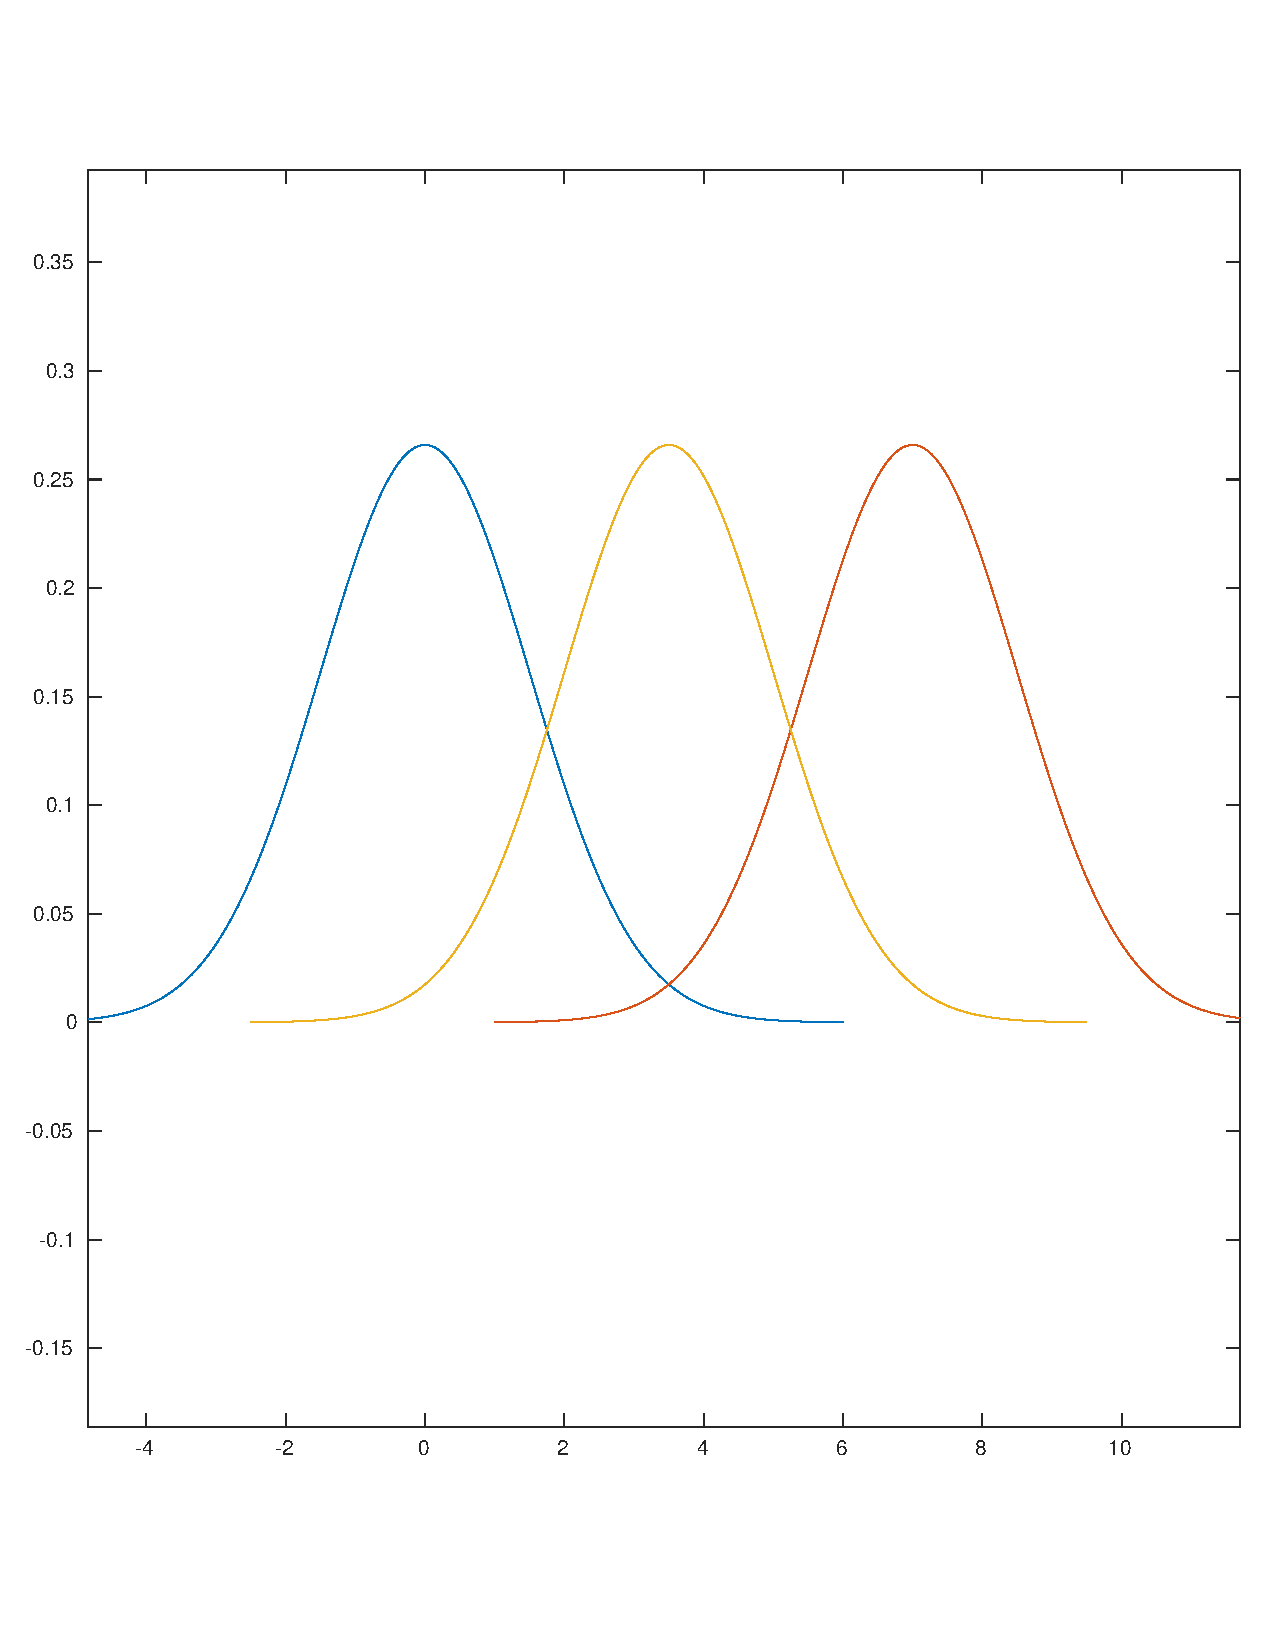
\includegraphics[width=0.7\textwidth, height=100px]{normal_distributions.pdf}                                                                  
		
	\end{center}
	\caption{Grundidee des Kalmanfilters}
	\label{fig:kernideeKalman}
	
\end{figure}

\section{Innovation}
Die Innovation des Kalmanfilters ist der Vergleich zwischen Messung und Schätzung des Kalmanfilters. 

\section{Parameter des Update Gain}
Die Standardabweichung der Messung so wie die der Schätzung.\\
Das Update Gain wird wie folgt berechnet: \~{}

\begin{equation}
K = \frac{(\bar{\sigma}_k)^2}{(\bar{\sigma}_k)^2 + (\tilde{\sigma}_k)^2}\\
\end{equation}

\section{Wertebereich des Update Gain}
Der Wertebereich des Gain ist normalisiert. $[0, 1]$ \\

\section{Eingrenzung des Mittelwertes einer Schätzung}

Der Mittelwert der \textbf{neuen Schätzung} $\hat{x}_k$ wird mittels des Gain $K$, der \textbf{vorherigen Schätzung} $\bar{x}_k$ und der \textbf{neuen Messung} $\tilde{x}_k$ berechnet.

\begin{equation}
\hat{x}_k = \bar{x}_k + K \left( \tilde{x}_k - \bar{x}_k \right) 
\end{equation}

\section{Berechnung der Varianz}
\begin{equation}
\hat{\sigma}^2_k = \left( 1 - K \right) (\bar{\sigma_k})^2
\end{equation}






